% e.g., http://adsabs.harvard.edu/abs/2014ApJ...790..127B

\documentclass[modern]{aastex62}
\usepackage{amsmath}

% Load common packages
% \usepackage{microtype}  % ALWAYS!
\usepackage{amsmath}
\usepackage{amsfonts}
\usepackage{amssymb}
\usepackage{booktabs}

\usepackage{graphicx}
\usepackage{color}

\graphicspath{{figures/}}

% \definecolor{cbblue}{HTML}{3182bd}
% \usepackage{hyperref}
% \definecolor{linkcolor}{rgb}{0.02,0.35,0.55}
% \definecolor{citecolor}{rgb}{0.45,0.45,0.45}
% \hypersetup{colorlinks=true,linkcolor=linkcolor,citecolor=citecolor,
%             filecolor=linkcolor,urlcolor=linkcolor}
% \hypersetup{pageanchor=true}

\newcommand{\documentname}{\textsl{Article}}
\newcommand{\sectionname}{Section}
\renewcommand{\figurename}{Figure}
\newcommand{\equationname}{Equation}
\renewcommand{\tablename}{Table}

% Missions
\newcommand{\project}[1]{\textsl{#1}}

% Packages / projects / programming
\newcommand{\package}[1]{\textsl{#1}}
\newcommand{\acronym}[1]{{\small{#1}}}
\newcommand{\github}{\package{GitHub}}
\newcommand{\python}{\package{Python}}
\newcommand{\emcee}{\project{emcee}}

% For referee
\newcommand{\changes}[1]{{\color{red} #1}}

% Stats / probability
\newcommand{\given}{\,|\,}
\newcommand{\norm}{\mathcal{N}}

% Maths
\newcommand{\dd}{\mathrm{d}}
\newcommand{\transpose}[1]{{#1}^{\mathsf{T}}}
\newcommand{\inverse}[1]{{#1}^{-1}}
\newcommand{\argmin}{\operatornamewithlimits{argmin}}
\newcommand{\mean}[1]{\left< #1 \right>}

% Unit shortcuts
\newcommand{\msun}{\ensuremath{\mathrm{M}_\odot}}
\newcommand{\kms}{\ensuremath{\mathrm{km}~\mathrm{s}^{-1}}}
\newcommand{\mps}{\ensuremath{\mathrm{m}~\mathrm{s}^{-1}}}
\newcommand{\pc}{\ensuremath{\mathrm{pc}}}
\newcommand{\kpc}{\ensuremath{\mathrm{kpc}}}
\newcommand{\kmskpc}{\ensuremath{\mathrm{km}~\mathrm{s}^{-1}~\mathrm{kpc}^{-1}}}

% Misc.
\newcommand{\bs}[1]{\boldsymbol{#1}}

% Astronomy
\newcommand{\DM}{{\rm DM}}
\newcommand{\feh}{\ensuremath{{[{\rm Fe}/{\rm H}]}}}
\newcommand{\df}{\acronym{DF}}
\newcommand{\logg}{\ensuremath{\log g}}
\newcommand{\Teff}{\ensuremath{T_{\textrm{eff}}}}

% TO DO
\newcommand{\todo}[1]{{\color{red} TODO: #1}}

\newcommand{\dr}[1]{\acronym{DR}#1}
\newcommand{\apogee}{\project{\acronym{APOGEE}}}
\newcommand{\sdss}{\project{\acronym{SDSS}}}
\newcommand{\sdssiv}{\project{\acronym{SDSS-IV}}}
\newcommand{\thejoker}{\project{The~Joker}}


\shorttitle{Stuff}
\shortauthors{Price-Whelan et al.}

\begin{document}

\title{Stellar and substellar companions in APOGEE DR16: \\
       Catalog of XX systems}

\author[0000-0003-0872-7098]{Adrian~M.~Price-Whelan}
\affiliation{Center for Computational Astrophysics, Flatiron Institute,
             Simons Foundation, 162 Fifth Avenue, New York, NY 10010, USA}
\email{aprice-whelan@flatironinstitute.org}
\correspondingauthor{Adrian M. Price-Whelan}

% \author[0000-0003-2866-9403]{David~W.~Hogg}
% \affiliation{Max-Planck-Institut f\"ur Astronomie,
%              K\"onigstuhl 17, D-69117 Heidelberg, Germany}
% \affiliation{Center for Cosmology and Particle Physics,
%              Department of Physics,
%              New York University, 726 Broadway,
%              New York, NY 10003, USA}
% \affiliation{Center for Data Science,
%              New York University, 60 Fifth Ave,
%              New York, NY 10011, USA}
% \affiliation{Flatiron Institute,
%              Simons Foundation,
%              162 Fifth Avenue,
%              New York, NY 10010, USA}

% \author[0000-0003-4996-9069]{Hans-Walter~Rix}
% \affiliation{Max-Planck-Institut f\"ur Astronomie,
%              K\"onigstuhl 17, D-69117 Heidelberg, Germany}

\author{Others}

\begin{abstract}
% Context
Binary star systems provide key context and constraints for nearly all subfields in astrophysics, from stellar evolution to XX to galaxy evolution.
% Aims
% Methods
% Results
% Conclusions
\end{abstract}

\keywords{}


\section{Introduction} \label{sec:intro}

A better understanding the formation and evolution of the popoulation of binary stars is important for all aspects of astrophysics, ... stellar-mass binary black hole mergers to stellar populations in high-redshift galaxies \citep[e.g.,][]{Breivik:2019, Rix:2019}.
This problem spans a wide range of timescales, wavelengths, and many current and near-future stellar surveys (Gaia, APOGEE, LAMOST, SDSS-V, etc.) have the capacity to deliver samples of binary stars and stellar companions orders of magnitude larger than are presently known, throughout all stages of stellar evolution.
The dream: combine all if this and learn about stellar evolution.
This has only been comprehensively done for a sample of a few hundred stars in solar neighborhood.

As a step towards large-scale population inference, we focus here on multi-epoch spectroscopic data from the APOGEE surveys.
The challenge: data are often sparse, most individual systems are not determined uniquely.
We have machinery to generate full samplings over orbital parameters for radial velocity data, under the assumptions listed in The Joker paper (SB1, etc.).
We run this sampler on all of APOGEE DR16 with some quality cuts and release the resulting catalog of posterior samples, along with some summary metadata for unimodal / uniquely determined orbits.

We use these samples to infer the companion period-eccentricity distribution over the HR diagram as an initial demonstration of hierarchical inference.


\section{Data} \label{sec:data}

We primarily use spectroscopic data from data release 16 (\dr{16}) of the
\apogee\ surveys (\citealt{Majewski:2017, Abolfathi:2017, DR16}).
\apogee\ is a component of the Sloan Digital Sky Survey IV (\sdssiv;
\citealt{Gunn:2006, Blanton:2017}) and the main goal is to survey the chemical
and dynamical properties of stars across much of the Milky Way disk by obtaining
high-resolution ($R \sim 22,500$) infrared ($H$-band) spectroscopy of hundreds
of thousands of stars.
The primary survey targets are selected with simple color and magnitude cuts,
but the survey uses fiber-plugged plates that leads to extremely nonuniform
coverage of the Galactic stellar distribution (see, e.g., Figure~1 in \citealt{DR16}).

\dr{16} is the first \sdss\ data release to contain \apogee\ data observed with
a clone of the \apogee\ spectrograph on the 2.5m du Point telescope at Las
Campanas Observatory, providing access to targets in the southern hemisphere.
For the first time, this data release also contains calibrated stellar
parameters for dwarf stars.
These two facts mean that \dr{16} contains nearly $3\times$ more sources with
calibrated stellar parameters than the previous public data release, \dr{14}
(see Section~4 of \citealt{DR16} for many more details about \apogee\ \dr{16}).

Most \apogee\ stars are observed multiple times in a set of time-resolved
``visits'' that are combined before determining stellar parameters and chemical
abundances.
While the visit spectra naturally provide time-domain velocity information about
sources, studying stellar multiplicity is not the primary goal of the survey:
The cadence and time baseline for a typical \apogee\ source is primarily
governed by trying to schedule a set number of visits determined by
signal-to-noise thresholds for the faintest targets in a given field.
A consequence of this strategy is that the time resolution and number of visits
for the vast majority of \apogee\ sources in \dr{16} is not sufficient for fully
determining companion orbital properties, as illustrated below.

\subsection{Quality cuts and defining a parent sample}

The primary goal of the catalog released with this \documentname\ is to provide
posterior samplings in Keplerian orbital parameters for all high-quality
\apogee\ sources in \dr{16} with multiple, well-measured radial velocities.
We therefore impose a set of quality cuts to sub-select \apogee\ \dr{16} sources
by rejecting sources or visits using the following \apogee\
bitmasks\footnote{https://www.sdss.org/dr16/algorithms/bitmasks/}:
\begin{itemize}
    \item Source-level (\texttt{allStar}) \texttt{STARFLAG} must not contain \texttt{VERY\_BRIGHT\_NEIGHBOR}, \texttt{SUSPECT\_RV\_COMBINATION} (bitmask value: 65544)
    \item Source-level (\texttt{allStar}) \texttt{ASPCAPFLAG} must not contain \texttt{TEFF\_BAD}, \texttt{LOGG\_BAD}, \texttt{VMICRO\_BAD}, \texttt{ROTATION\_BAD}, \texttt{VSINI\_BAD} (bitmask value: 1141309440)
    \item Visit-level (\texttt{allVisit}) \texttt{STARFLAG} must not contain \texttt{VERY\_BRIGHT\_NEIGHBOR}, \texttt{SUSPECT\_RV\_COMBINATION}, \texttt{LOW\_SNR}, \texttt{PERSIST\_HIGH}, \texttt{PERSIST\_JUMP\_POS}, \texttt{PERSIST\_JUMP\_NEG} (bitmask value: 78360)
\end{itemize}
These bitmasks are designed to remove the most obvious data reduction or calibration failures that would directly impact the visit-level radial velocity determinations.
However, we later impose a stricter set of quality masks when showing results in \sectionname~\ref{sec:TODO}.
After applying the above masks, we additionally reject any source with $<3$
visits.
Our final parent sample contains $232,531$ unique sources, cut down from the
$437,485$ unique sources in all of \apogee\ \dr{16}.
Of the $\approx$$200,000$ removed sources, the vast majority were removed because they had $<3$ visits ($\approx$$17,000$ were removed by the quality cuts).

% Notebook: Figure-DR16-statistics.ipynb
\begin{figure}[th]
\begin{center}
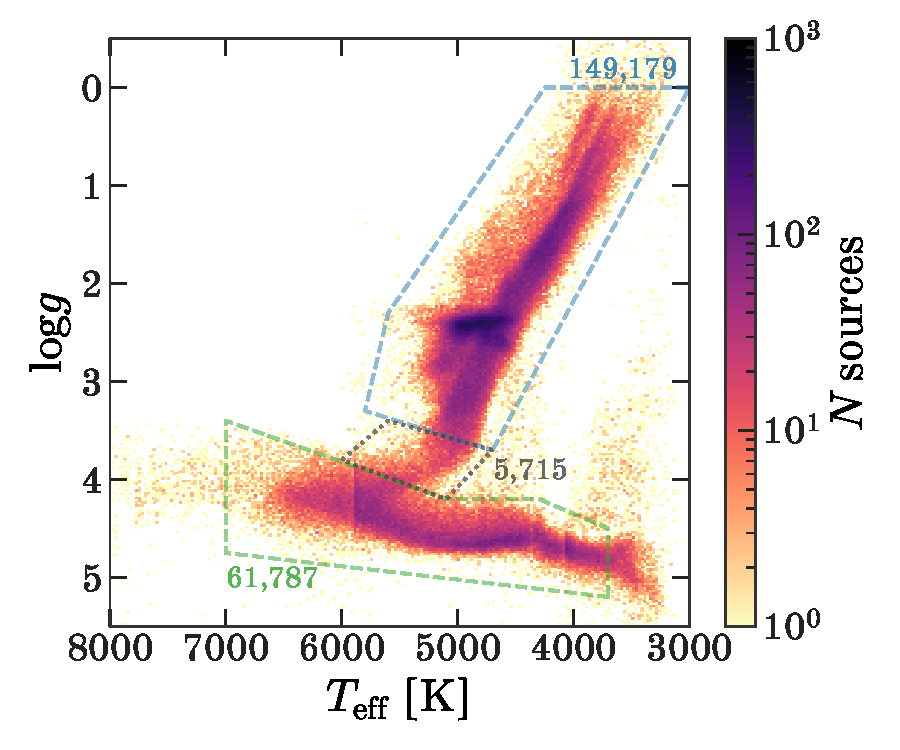
\includegraphics[width=0.7\textwidth]{specHR.pdf}
\end{center}
\caption{%
Two spectroscopic stellar parameters---effective temperature, $T_{\rm eff}$, and
log-surface gravity, $\log g$---of \apogee\ \dr{16} sources that pass our
quality cuts; These sources represent our ``parent sample.''
The pixel coloring indicates the number of sources in each bin of stellar
parameters.
The outlined regions roughly identify the red giant branch (upper polygon,
blue), subgiant branch (middle polygon, black), and (FGK-type) main sequence
(lower polygon, green).
The numbers next to each selection polygon indicate the number of sources in
each.
\label{fig:specHR}
}
\end{figure}

% Notebook: Figure-DR16-statistics.ipynb
\begin{figure}[th]
\begin{center}
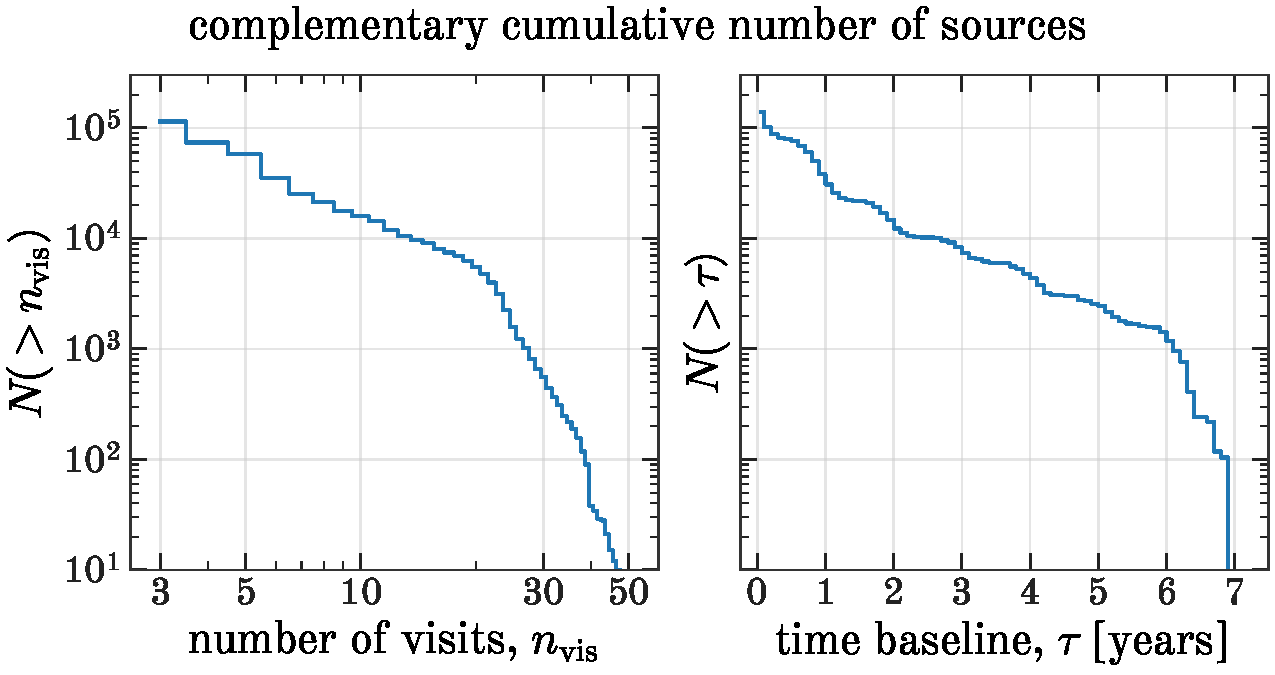
\includegraphics[width=1\textwidth]{visitstats.pdf}
\end{center}
\caption{%
Derp derp derp.
\label{fig:visitstats}
}
\end{figure}

Figure~\ref{fig:specHR} shows the number of sources in our parent sample---i.e.
\apogee\ sources with 3 or more visits that pass the quality cuts described
above---as a function of spectroscopic stellar parameters $T_{\rm eff}$,
effective temperature, and $\log g$, log-surface gravity.
While the majority of sources appear to be giant-branch stars ($>150,000$), a
substantial number of main sequence stars are present ($>60,000$) thanks to the
\apogee\ data reduction pipeline improvements for \dr{16}.
Figure~\ref{fig:visitstats} shows some statistics about the time coverage of the
visits for sources in our parent sample:
\begin{itemize}
    \item $\approx$70\% ($\approx$92\%) of sources have $<5$ ($<10$) visits, and
    $17,786$ sources have 10 or more visits,
    \item $\approx$50\% ($\approx$84\%) of sources have time baselines $<56~{\rm days}$ ($<1~{\rm year}$), and $9,743$ sources have time baselines $>1000~{\rm days}$.
\end{itemize}


\subsection{Visit velocity error calibration} \label{sec:visitcalib}

Visit velocity errors underestimated, so we perform our own calibration.

Describe exoplanet survey crossmatch and calibration bullshit.

This ends up being conservative: we effectively force low SNR visit to a SNR-dependent threshold rv err, high SNR stars get adjusted too with a global floor to RV error.

Figure: raw visit errors vs. SNR and then adjusted visit errors


\section{Methods} \label{sec:methods}

Describe The Joker.

Describe robust constant fit.

\subsection{Caveats} \label{sec:caveats}

Where we will fail:

Systems with large systemic velocity (dwarf satellites)

Triple systems

\section{A catalog of binary stars} \label{sec:catalog}

Any catalog will have some arbitrary cuts. Here we cut on likelihood ratio of binary star model vs. constant model (not fully marginal likelihoods, so cut won't be at 0!).

We find XX stars with companions - show simple plots over HR diagram for cuteness.

Gold sample: phase coverage statistics?

TODO: what about bimodal samplings, or samplings with small range in ln-period?

Figure: Some cute examples

Figure: Fraction of stars with companions over HR diagram

\section{Inferring shit with a hierarchical model} \label{sec:Pe}

\begin{align}
    z &= \ln\,P\\
    \bs{\theta} &= (z, e)\\
    \bs{\alpha} &= (k, z_0, \alpha_0)\\
    p(\bs{\theta} \given \bs{\alpha}) &= p(z) \, p(e \given z)\\
    p(z) &= \norm\left(z \given \mu_z, \sigma_z^2 \right)\\
    p(e \given z) &= \alpha(z) \, p_1(e) + (1-\alpha(z)) \, p_2(e)\\
    f(z\,;\,k,z_0) &= \frac{1}{1 + e^{-k\,(z - z_0)}}\\
    \alpha(z \,;\, k, z_0, \alpha_0) &= (1-\alpha_0) \, f(z \,;\, k, z_0) + \alpha_0\\
    p_1(e) &= B(e \given a_1, b_1)\\
    p_2(e) &= B(e \given a_2, b_2)
\end{align}

\begin{align}
    p(D \given \bs{\alpha}) &= \int \dd\bs{\theta} \,
        p(D \given \bs{\theta}) \, p(\bs{\theta} \given \bs{\alpha})\\
    &\approx \frac{\mathcal{Z}}{K} \sum_k^K
        \frac{p(\bs{\theta}_k \given \bs{\alpha})}
            {p(\bs{\theta}_k \given \bs{\alpha}_0)}\\
    \bs{\theta}_k &\sim p(\bs{\theta} \given D, \bs{\alpha}_0)
\end{align}

- Period, eccentricity distributions
- Mass-ratio distribution
     - Use C,N abundances for RGB and logg, teff, fe/h for main sequence
     - Calibrate against asteroseismology / APOKASC


Lars: "Any idea of the incidence of stars which did an engulfment on their way UP the RGB from the Luminosity of the clump to that of the RGB TIP? "

% Note: some or all of these may be broken out into separate papers!

% \subsection{Companions along the RGB}
% Compare RGB vs. RC - see engulfment?
%
% \subsection{Brown dwarfs}
% So many!
%
% \subsection{Binary population statistics}
% Simple hierarchical inference?
%
% \subsection{TRGB asteroseismology}
%
% \subsection{Binary star populations in open clusters}
%
% \subsection{Binary star populations in globular clusters}

% Ack: Lars Bildsten


\software{
    Astropy \citep{astropy, astropy:2018},
    emcee \citep{emcee},
    gala \citep{gala},
    IPython \citep{ipython}
}

\bibliographystyle{aasjournal}
\bibliography{dr16vac}

\end{document}
